\section{Meta-Heuristic Charging Stations Placement}
\label{sec:5_3_mh_placement}
In this sections I explain the ratio behind the charging station placement. Indeed, in the previous section I described the structure and simulation policies, while now I define an important environmental variable that will be deeply studied in chapters \mc{references}. I remind that from the rental booking trace, I extrapolate the service area and I divide it into square zones of 500 m of side length. Then, using the number of parking or the average parking time for each zone, the simulator choose which zones equip with a charging station.

\subsection{Problem formalization}
Given a number of charging station $N$, the first objective is to place them in the city area so to let all rentals feasible, i.e., to find a charging stations placement so that
\[
c(a,t_e(i))>0\ \forall a \in \mathcal{A}, \forall  i \in \mathcal{I}
\]
Since I do not make any assumption on the set of trips $\mathcal{I}$, I cannot know a-priori if a solution exists and provide an analytical general solution. Moreover the number of candidate solutions increases as the binomial coefficient ${\left\vert{\mathcal{Z}}\right\vert}\choose\ N$, making ineffective to numerically compute all possibilities. Instead, I will provide a class of greedy algorithms and analyse the performance in our specific cases of $\mathcal{I}$.
In details, each zone $z\in\mathcal{Z}$ is assigned a likelihood $l_z \geq 0$.
We then solve the problem of finding the subset of $N$ zones that maximizes the total likelihood. In formulas, 
$$\max \sum_{z\in\mathcal{Z}} cs(z)l_z$$

subject to:
$$\sum_{z\in\mathcal{Z}} cs(z) = N$$
$$cs(z)\in \{0,1\},  \forall z \in \mathcal{Z}$$

The above optimization problem can be solved by greedily choosing the top $N$ zones, ordered in decreasing likelihood. We compare the performance of different placement algorithms based on different definition of the likelihood.
\begin{itemize}
	\item{\it Random placement}: $l_z$ is an independent and identical distributed random uniform variable, so that charging stations result placed at random;
	\item{\it Average parking time}: $l_z$ is the average parking duration in $z$ as recorded in the trace;
	\item{\it Total number of parkings}: $l_z$ is the total number of parking events recorded in $z$ in the trace;
	\item{\it Total parking time}: $l_z$ is the total parking time accumulated in $z$ by all cars recorded in the trace. In each zone, it is the product of the two previous metrics.
\end{itemize}
Those heuristics are driven by the intuition that placing charging stations in those zones where cars are parked for long time (average parking time) or frequently parked (total number of parkings) could improve system performance.


\begin{figure}[th]
	\centering     %%% not \center
	\subfloat[\centering Turin]{{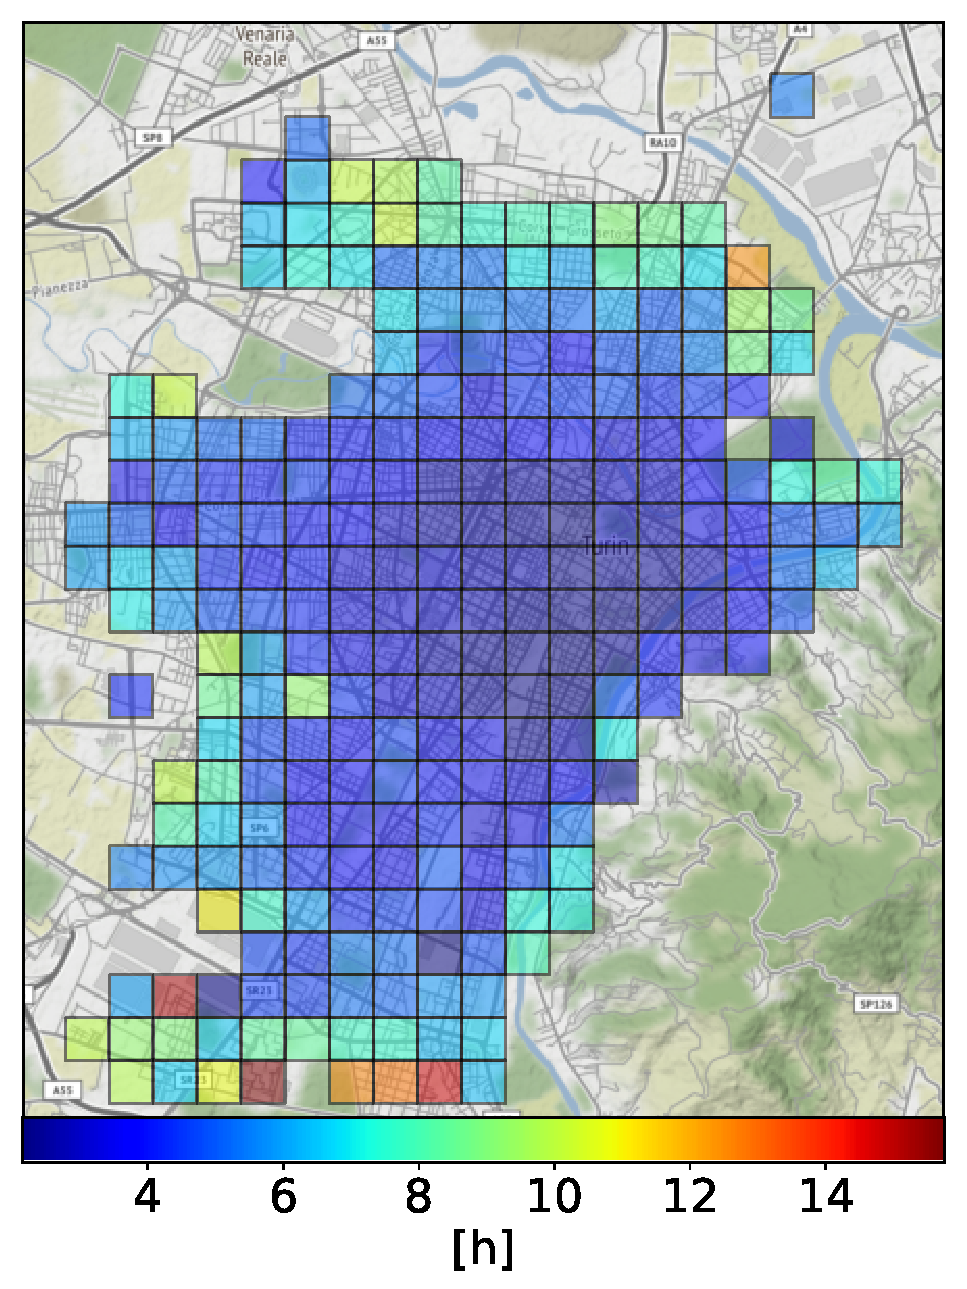
\includegraphics[width=0.24\columnwidth]{images_pdf/Torino_AvgTime.pdf}}\label{fig:5_4_ap_turin}}
	\quad
	\subfloat[\centering Vancouver]{{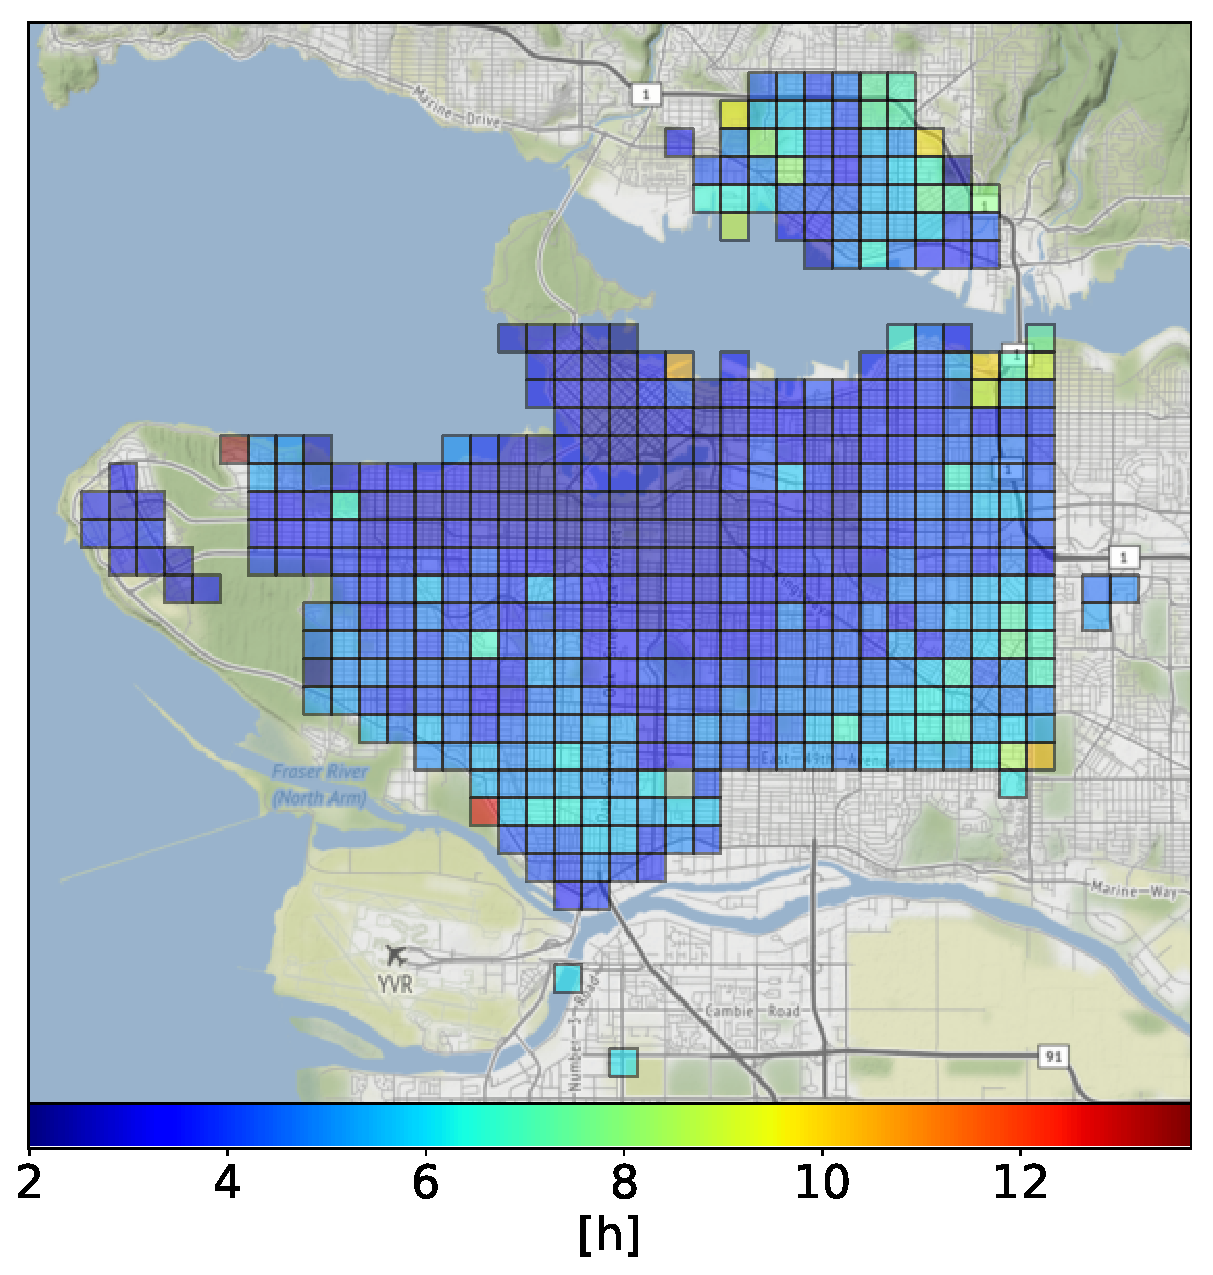
\includegraphics[width=0.30\columnwidth]{images_pdf/Vancouver_AvgTime.pdf}}\label{fig:5_4_ap_vancouver}}
	\quad
	\subfloat[\centering Berlin]{{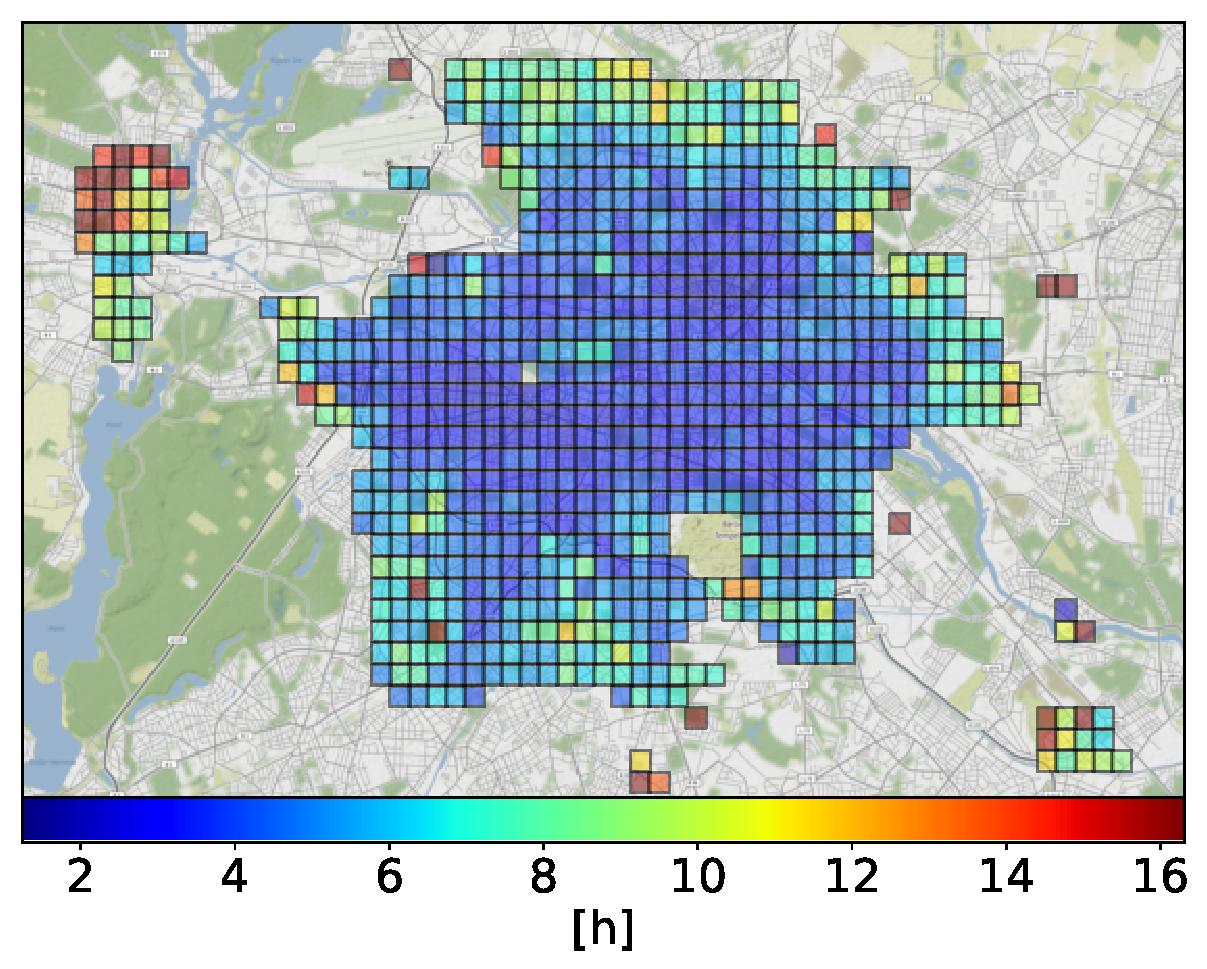
\includegraphics[width=0.39\columnwidth]{images_pdf/Berlino_AvgTime.pdf}}\label{fig:5_4_ap_berlin}}%
	\caption{Distribution of average parking time in Turin, Vancouver and Berlin}
	\label{fig:5_4_heatmap_avgparking}
\end{figure}

I order to show the differences between the likelihoods $l_z$ criteria, figures \ref{fig:5_4_heatmap_avgparking} where $l_z$ is depicted for Turin (\ref{fig:5_4_ap_turin}), Vancouver (\ref{fig:5_4_ap_vancouver}) and Berlin (\ref{fig:5_4_ap_berlin}). The first two cities were deeply characterized in chapters \ref{chap:3_charact} and \ref{chap:4_cs_comparison}, while Berlin, as I will show, presents some interesting spatial distribution. In all the figures, in particular, the more the zone is red, the higher is $l_z$. It means that the \emph{redest} zones will be the first to host a charging station.

In first approach it is possible to se how, in all figures, the heuristic \textit{Average parking time} is mainly spread in city peripheries. It means that the cars spend a lot of times parked far from city centre. This peculiarity can be imputed to commuting patterns: as figure \ref{fig:bookingsweek} points out, two peaks are present in the users' demand. In particular the evening peak catches the back-home commuting which, usually is directed to high-density residential area located in periphery. This, joint with the low business-days night demand, leads to users to leave cars parked in that areas all night long.


\begin{figure}[th]
	\centering     %%% not \center
	\subfloat[\centering Turin]{{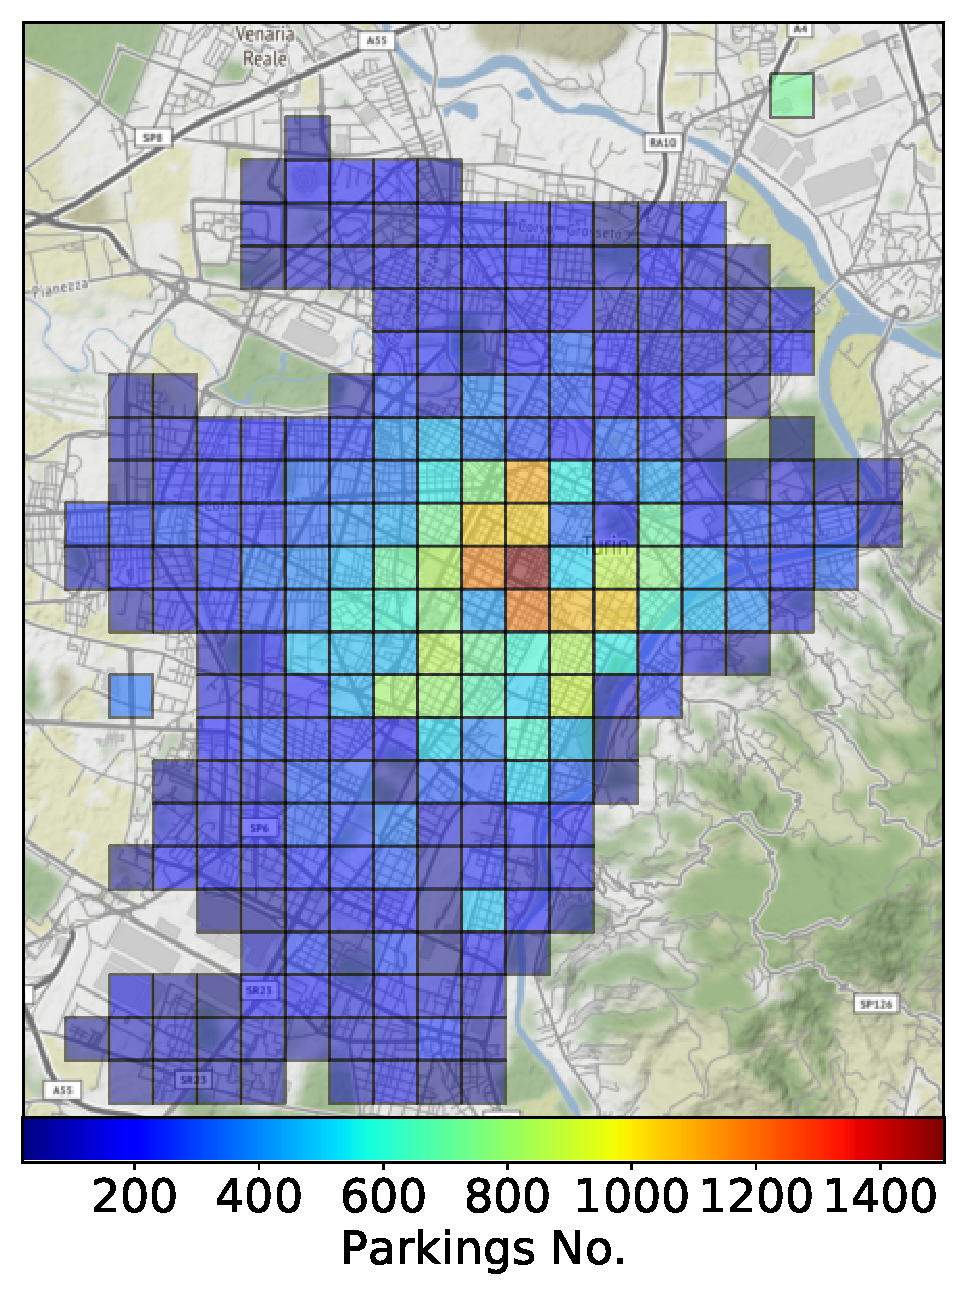
\includegraphics[width=0.24\columnwidth]{images_pdf/Torino_NParkings.pdf}}\label{fig:5_4_np_turin}}
	\quad
	\subfloat[\centering Vancouver]{{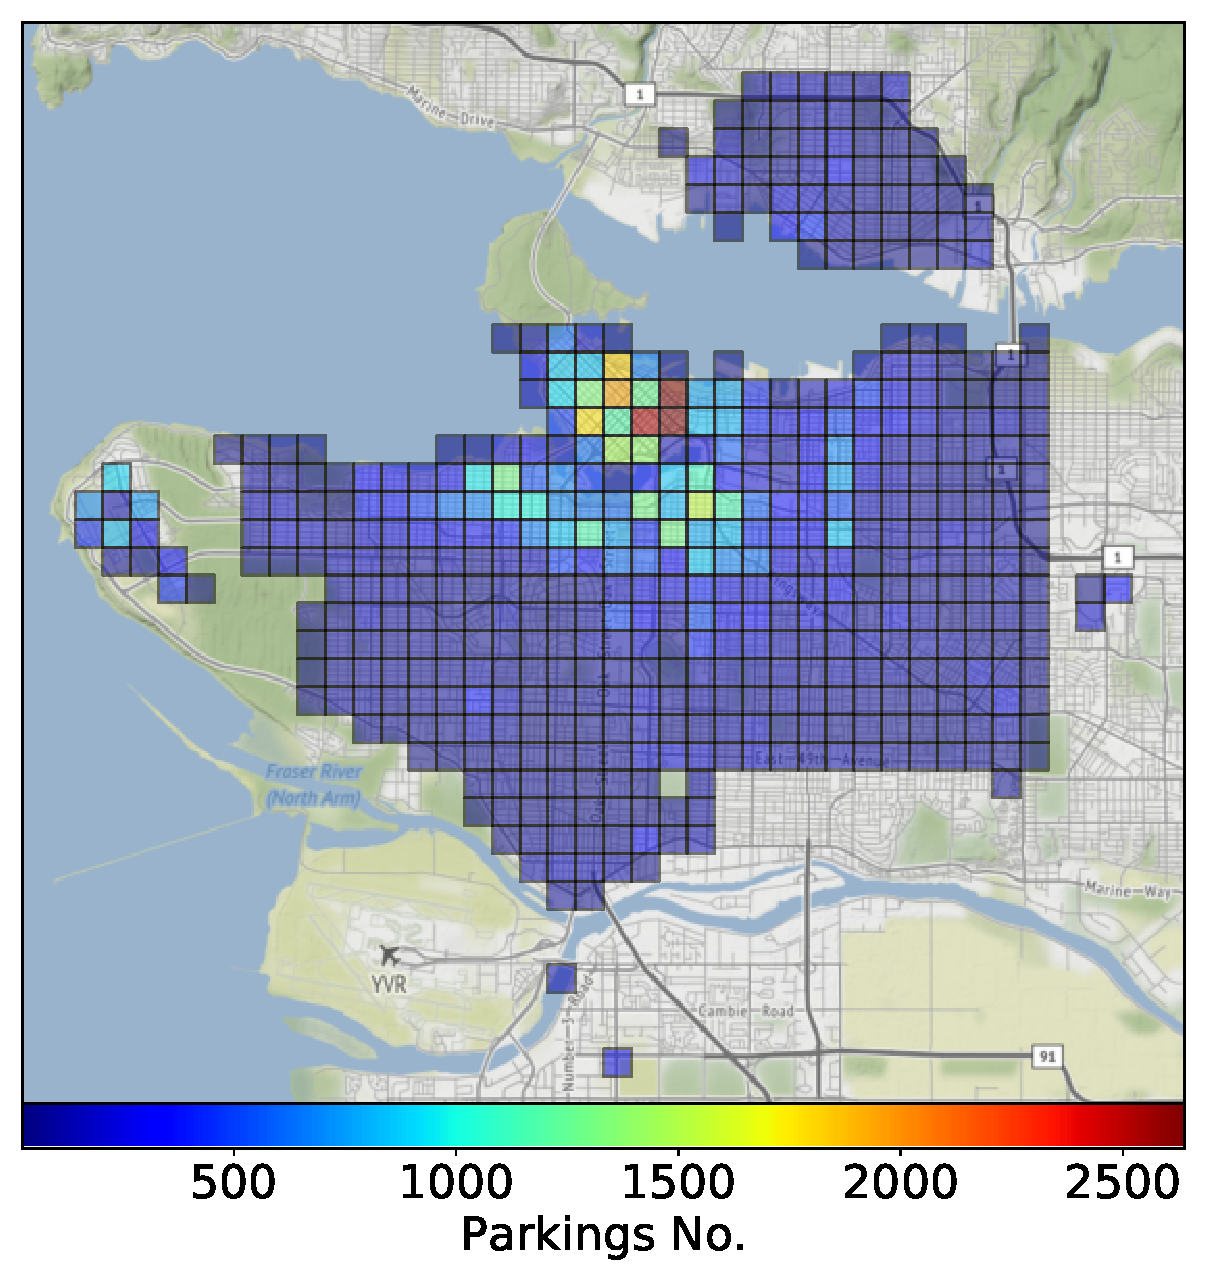
\includegraphics[width=0.30\columnwidth]{images_pdf/Vancouver_NParkings.pdf}}\label{fig:5_4_np_vancouver}}
	\quad
	\subfloat[\centering Berlin]{{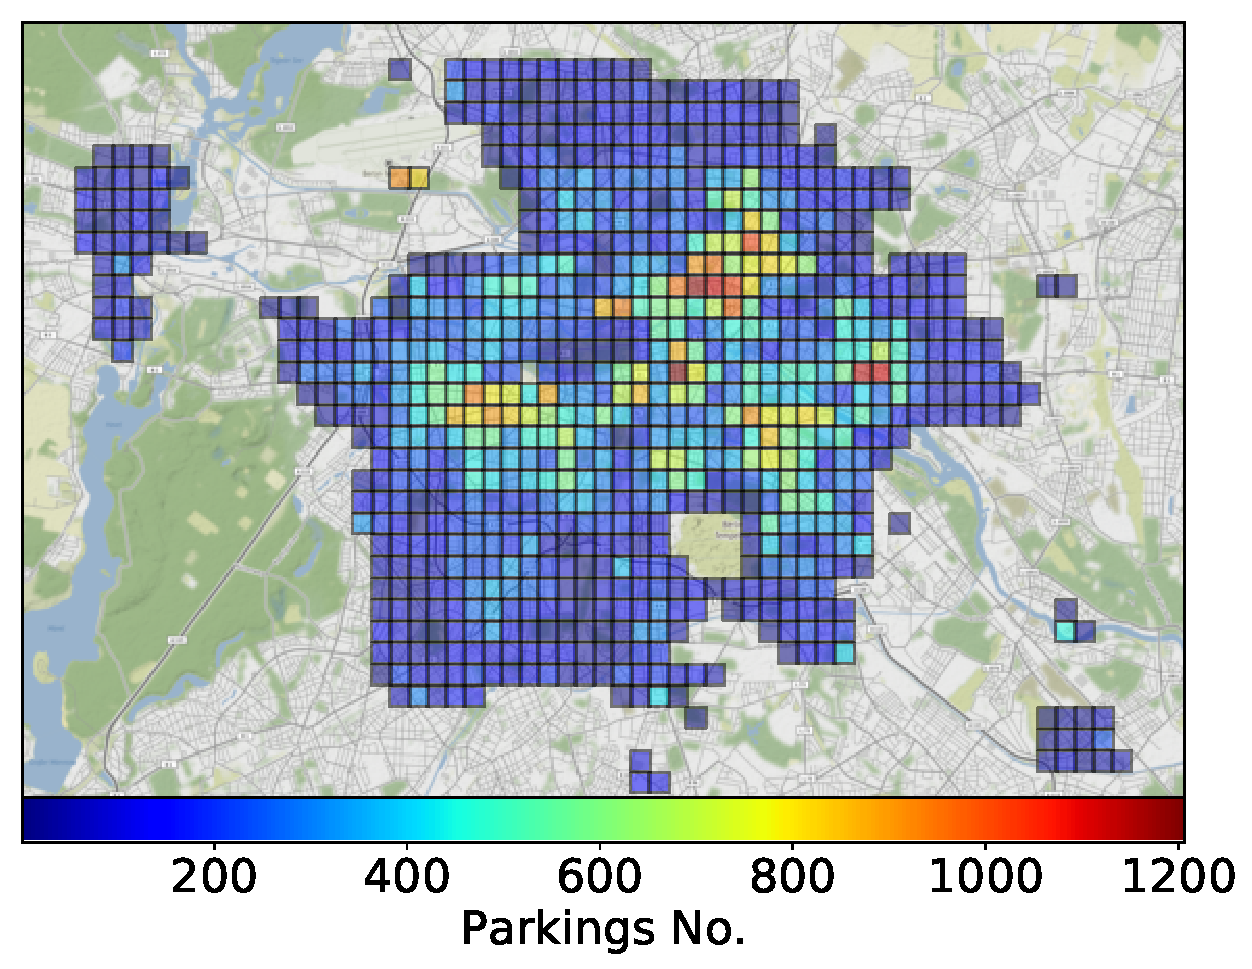
\includegraphics[width=0.40\columnwidth]{images_pdf/Berlino_NParkings.pdf}}\label{fig:5_4_np_berlin}}%
	\caption{Distribution of number of parking in Turin, Vancouver and Berlin}
	\label{fig:5_4_heatmap_numparking}
\end{figure}

Figure \ref{fig:5_4_heatmap_numparking} depicts the number of parking in each zone, for Turin (\ref{fig:5_4_np_turin}), Vancouver (\ref{fig:5_4_np_vancouver}) and Berlin (\ref{fig:5_4_np_berlin}). Reminding that more parkings means an higher zone attractiveness,
 it is possible to notice how the zones with the highest number of parking concentration zones are delimited in particular areas. For example figure \ref{fig:5_4_np_turin} shows how most frequented areas are downtown in correspondence of the two main train stations and the airport. A similar pattern can be spot in figure \ref{fig:5_4_np_vancouver}. Contrary, Berlin presents at least three attractive areas. This is mainly due to the biggest operative area and, probably, to the differentiation of business areas.
 
For completeness, I report in figure \ref{fig:5_4_heatmap_sumtime} the \textit{Total parking time} likelihood. It appears to smooth the behaviour of the previous two metrics.

\begin{figure}[th]
	\centering     %%% not \center
	\subfloat[\centering Turin]{{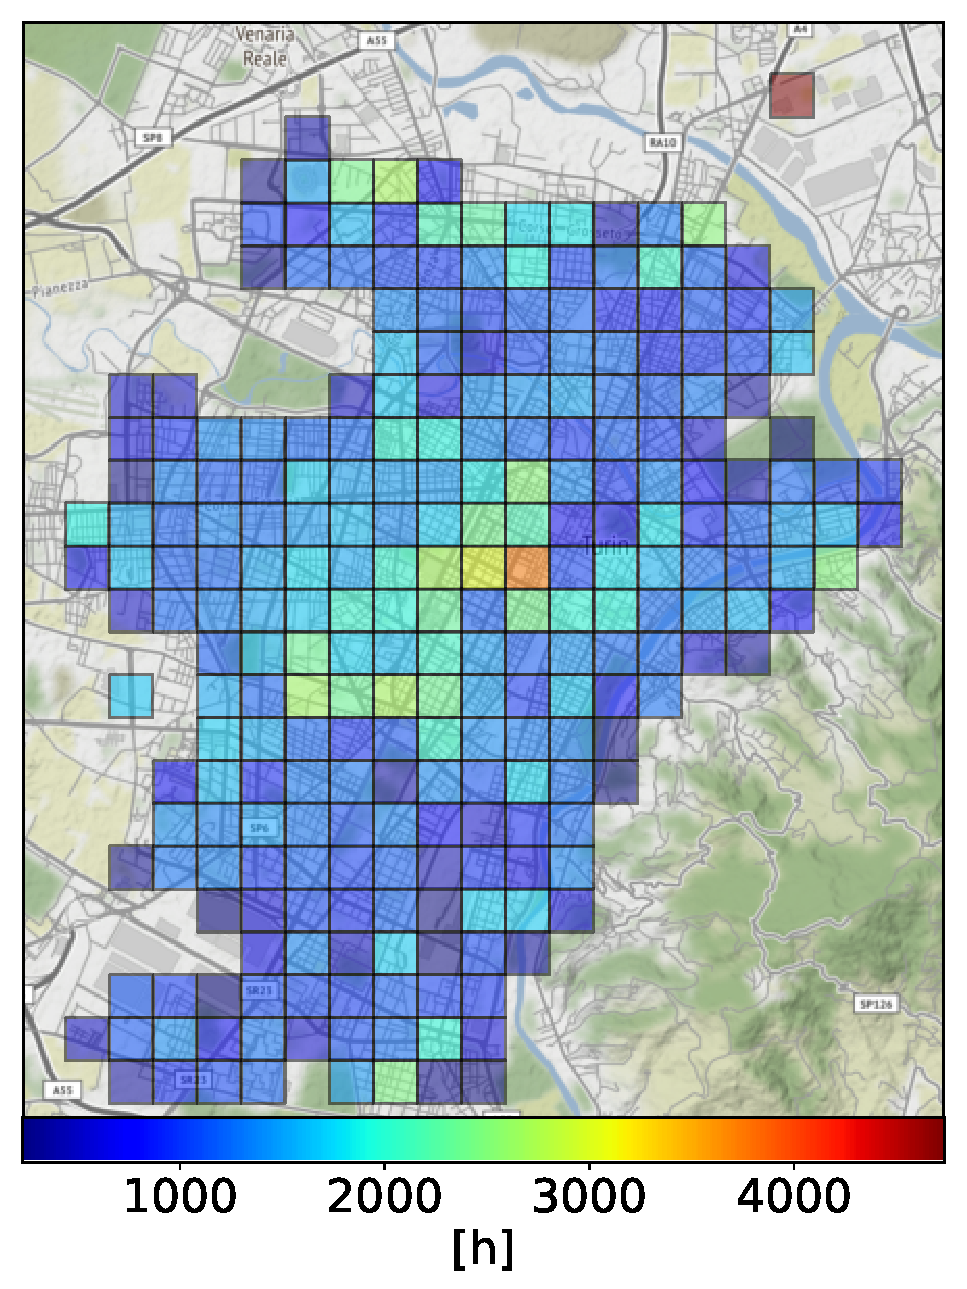
\includegraphics[width=0.24\columnwidth]{images_pdf/Torino_SumTime.pdf}}\label{fig:5_4_st_turin}}
	\quad
	\subfloat[\centering Vancouver]{{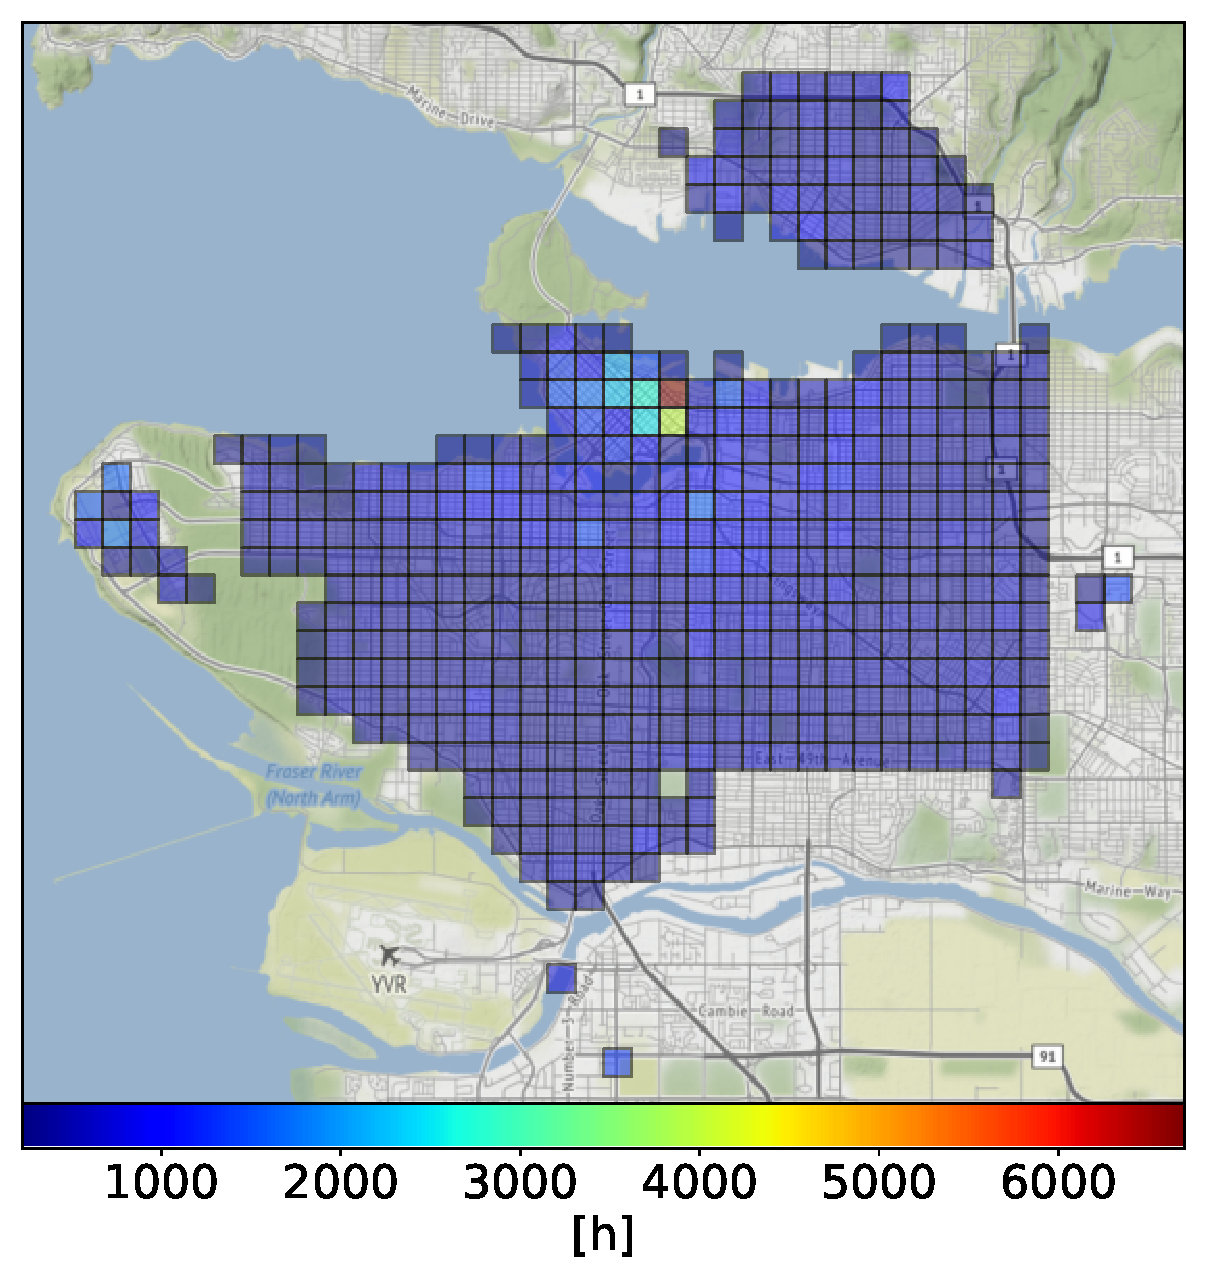
\includegraphics[width=0.30\columnwidth]{images_pdf/Vancouver_SumTime.pdf}}\label{fig:5_4_st_vancouver}}
	\quad
	\subfloat[\centering Berlin]{{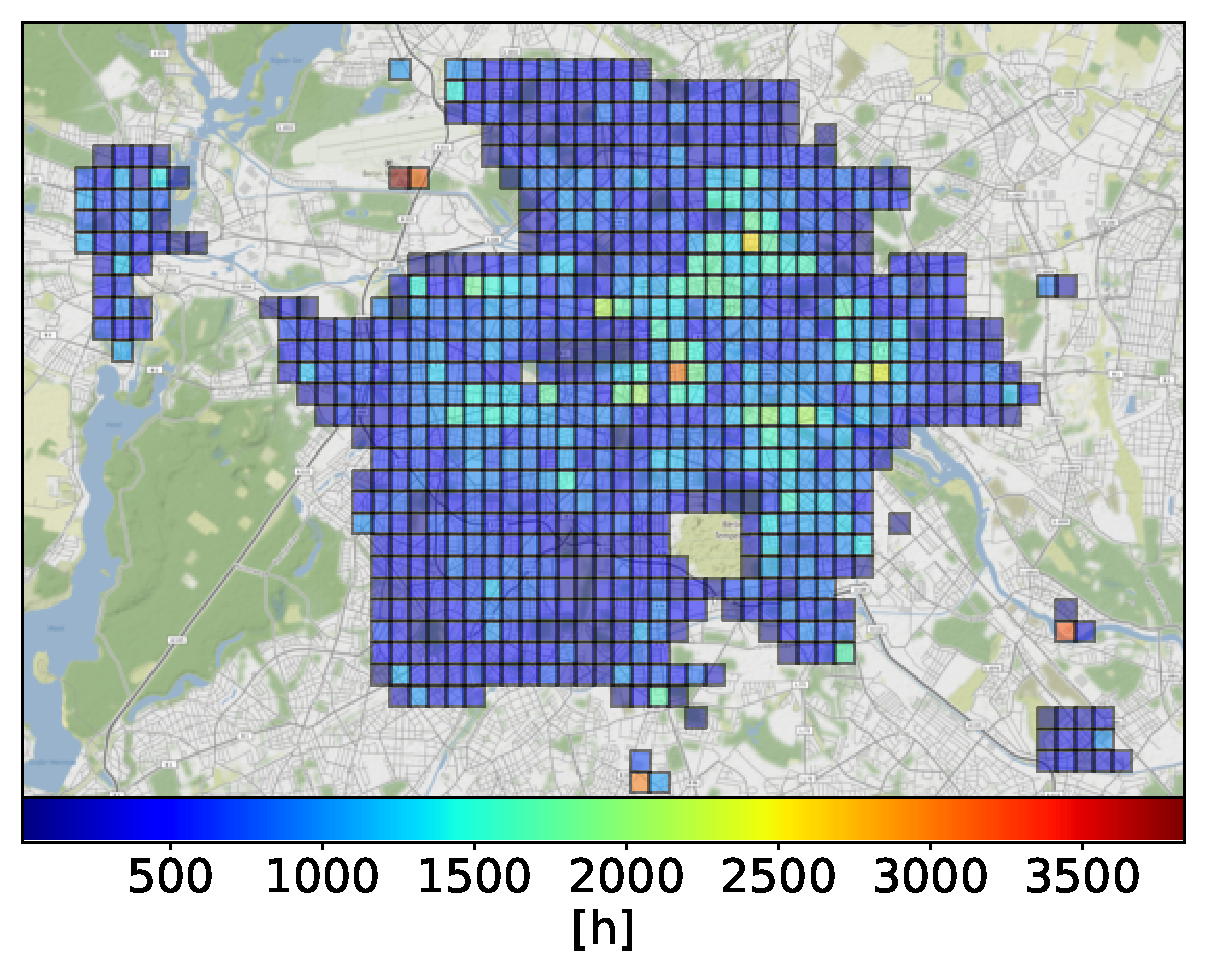
\includegraphics[width=0.39\columnwidth]{images_pdf/Berlino_SumTime.pdf}}\label{fig:5_4_st_berlin}}%
	\caption{Distribution of total parking time in Turin, Vancouver and Berlin}
	\label{fig:5_4_heatmap_sumtime}
\end{figure} 

This brief catheterization shows how  different cities can have different spatial characterization and thus different charging station placements. However those characterization will be deepened in chapters \mc{captoli}.
